\documentclass[11pt]{article}
% Packages
% ---
\usepackage{listings} % Source code formatting and highlighting 
\usepackage{fullpage}
\usepackage{color}
\usepackage{xcolor}
\usepackage{hyperref}
\usepackage{xparse}
\usepackage{graphicx}

% Title variables
% --- 
\author{ 
	Dylan Phelan \\ 
	Working With Corpora \\ 
	Professor Gregory Crane 
}
\title{Assignment 4}
\date{October 6, 2018}
 
% Definitions
% ---- 
% Colors
\definecolor{lightCyan}{HTML}{62929E}
\definecolor{khaki}{HTML}{C3B299}
\definecolor{orange}{HTML}{FFA552}
\definecolor{gray}{HTML}{A1A0AA}
\definecolor{olive}{HTML}{516D27}
% Envs
\newenvironment{solution}{
	\vspace{10px}\noindent\emph{Solution:}
}{
	\vspace{10px}
}
% Cmds
\newcommand{\codeword}[1]{
	\texttt{\textcolor{lightCyan}{#1}}
}
% Define our code blocks
\lstset{
	frame=tb,
	language=Python,
	aboveskip=2mm,
	belowskip=2mm,
	showstringspaces=false,
	columns=flexible,
	basicstyle={\small\ttfamily},
	numberstyle=\textcolor{khaki},
	keywordstyle=\textcolor{orange},
	commentstyle=\textcolor{gray},
	stringstyle=\textcolor{olive},
	breaklines=true,
	breakatwhitespace=true,
	tabsize=3
}

 
\begin{document}
\maketitle

\section*{Exercises for Chapter 5: Categorizing and Tagging Words}
\subsection*{Problem 19}

The evaluate() method works out how accurately the tagger performs on this text. For example, if the supplied tagged text was [('the', 'DT'), ('dog', 'NN')] and the tagger produced the output [('the', 'NN'), ('dog', 'NN')], then the score would be 0.5. Let's try to figure out how the evaluation method works:

\begin{enumerate}
	
	\item A tagger \codeword{t} takes a list of words as input, and produces a list of tagged words as output. However, \codeword{t.evaluate()} is given correctly tagged text as its only parameter. What must it do with this input before performing the tagging?
	
	\item Once the tagger has created newly tagged text, how might the evaluate() method go about comparing it with the original tagged text and computing the accuracy score?
	
	\item Now examine the source code to see how the method is implemented. Inspect nltk.tag.api.\_\_file\_\_ to discover the location of the source code, and open this file using an editor (be sure to use the api.py file and not the compiled api.pyc binary file).
	
\end{enumerate}

\begin{solution}
	
	\begin{enumerate}
		
		\item In order for \codeword{t.evaluate()} to tag a particular text, it has to first split each term from its tagged counterpart as provided in our supplied tagged text.
		
		\item After the tagger has generated it's tagged version of the text (or simultaneously as it's computing those tags) the tagger can compare for correctness each computed tag with the originally provided tag, calculating the percentage of tags that it got correct.
		
		\item Below you'll see the source code found in \codeword{api.py}:
		
	\end{enumerate}	
	
	\begin{lstlisting}
		def evaluate(self, gold):
			"""
			Score the accuracy of the tagger against the gold standard.
			Strip the tags from the gold standard text, retag it using
			the tagger, then compute the accuracy score.
			
			:type gold: list(list(tuple(str, str)))
			:param gold: The list of tagged sentences to score the tagger on.
			:rtype: float
			"""
			
			tagged_sents = self.tag_sents(untag(sent) for sent in gold)
			gold_tokens = list(chain(*gold))
			test_tokens = list(chain(*tagged_sents))
			return accuracy(gold_tokens, test_tokens)
	\end{lstlisting}

\end{solution} 


\newpage
\subsection*{Problem 20}

Write code to search the Brown Corpus for particular words and phrases according to tags, to answer the following questions:

\begin{enumerate}

	\item Produce an alphabetically sorted list of the distinct words tagged as MD.
	
	\item Identify words that can be plural nouns or third person singular verbs (e.g. deals, flies).
	
	\item Identify three-word prepositional phrases of the form IN + DET + NN (eg. in the lab).
	
	\item What is the ratio of masculine to feminine pronouns?

\end{enumerate}

\begin{solution}
	
	Console print outs corresponding to my answers: 
	
	\begin{lstlisting}
		--- 1: A sample of unique instances of MD
		["c'n", 'can', 'colde', 'could', 'dare', 'kin', 'maht', 'mai', 'may', 'maye'] ...
		
		--- 2: A sample of words that can be plural nouns or 3rd person singular verbs
		['likes', 'bases', 'signals', 'marches', 'views', 'addresses', 'knocks', 'points', 'loves', 'crops'] ...
		
		--- 3: A sample of trigrams of form IN + DET + NN
		['of the election', 'for the manner', 'in the election', 'to the end', 'on a number', 'of the law', 'through the welfare', 'in the state', 'with the exception', 'in the future'] ...
		
		--- 4: Ratio of masculine to feminine (based on universal tagset)
		masc_count:  12816
		fem_count:  4108
		3.1197663096397275
	\end{lstlisting}
	
	Actual code: 

	\begin{lstlisting}
		import nltk 
		from nltk.corpus import brown
		import functools
		# 1. Produce an alphabetically sorted list of the distinct words tagged as MD.
		def unique_instances_of_pos(tagged_text, pos): 
			pos_terms = [term.lower() for (term, tag) in tagged_text if tag == pos]
			pos_sorted_instances = sorted(list(set(pos_terms)))
			return pos_sorted_instances
		
		# 2. Identify words that can be plural nouns or third person singular verbs (e.g. deals, flies).
		def words_with_both_pos(tagged_text, pos1, pos2): 
			terms_with_pos1 = set()
			terms_with_pos2 = set()
			for (word, tag) in tagged_text: 
				if tag == pos1: 
					terms_with_pos1.add(word.lower())
				if tag == pos2: 
					terms_with_pos2.add(word.lower())
			terms_with_both = list(terms_with_pos1.intersection(terms_with_pos2))
			return terms_with_both
		
		# 3. Identify three-word prepositional phrases of the form IN + AT + NN (eg. in the lab).
		def trigams_with_pos(tagged_text, pos1, pos2, pos3): 
			trigrams = nltk.trigrams(tagged_text)
			trigrams_with_all_pos = [f"{tri[0][0]} {tri[1][0]} {tri[2][0]}"for triin nltk.trigrams(tagged_text) if tri[0][1] == pos1 and tri[1][1] == pos2 and tri[2][1] == pos3]
			return trigrams_with_all_pos
		
		# 4. What is the ratio of masculine to feminine pronouns?
		# Known masc and fem pronouns based on an exploration of the brown text we care about
		masc_pronouns = ["his", "hisself", "him", "himself", "he", "hymselfe", "hym", "'im", "himselfe"]
		fem_pronouns = ["herself", "her", "hers", "she"]
		
		def masc_fem_count_fn (count_tuple, pronoun): 
		(masc_count, fem_count) = count_tuple;
			if pronoun in masc_pronouns:
				return (masc_count + 1, fem_count)
			elif pronoun in fem_pronouns:
				return (masc_count, fem_count + 1)
			else: 
				return (masc_count, fem_count) 
		
		def ratio_masc_fem_pronouns(tagged_text):
			pronouns = [term.lower() for (term, tag) in nltk.corpus.brown.tagged_words(tagset="universal") if tag == "PRON"]
			(masc_count, fem_count) = functools.reduce(masc_fem_count_fn, pronouns, (0,0))
			print("masc_count: ", masc_count)
			print("fem_count: ", fem_count)
			ratio_masc_to_fem = masc_count/fem_count; 
			return ratio_masc_to_fem
		
		if __name__ == '__main__':
			brown_tagged = brown.tagged_words();
			sample_number = 10
			print("--- 1: A sample of unique instances of MD")
			print(unique_instances_of_pos(brown_tagged, "MD")[:sample_number], "...")
			print("\n--- 2: A sample of words that can be plural nouns or 3rd person singular verbs")
			print(words_with_both_pos(brown_tagged, "NNS", "VBZ")[:sample_number], "...")
			print("\n--- 3: A sample of trigrams of form IN + DET + NN")
			print(trigams_with_pos(brown_tagged, "IN", "AT", "NN")[:sample_number], "...")
			print("\n--- 4: Ratio of masculine to feminine (based on universal tagset)")
			print(ratio_masc_fem_pronouns(brown.tagged_words(tagset="universal")))
	\end{lstlisting}
	
\end{solution} 


\newpage
\subsection*{Problem 26}

 4.1 plotted a curve showing change in the performance of a lookup tagger as the model size was increased. Plot the performance curve for a unigram tagger, as the amount of training data is varied.

\begin{solution}
	
	\hspace*{-50pt}
	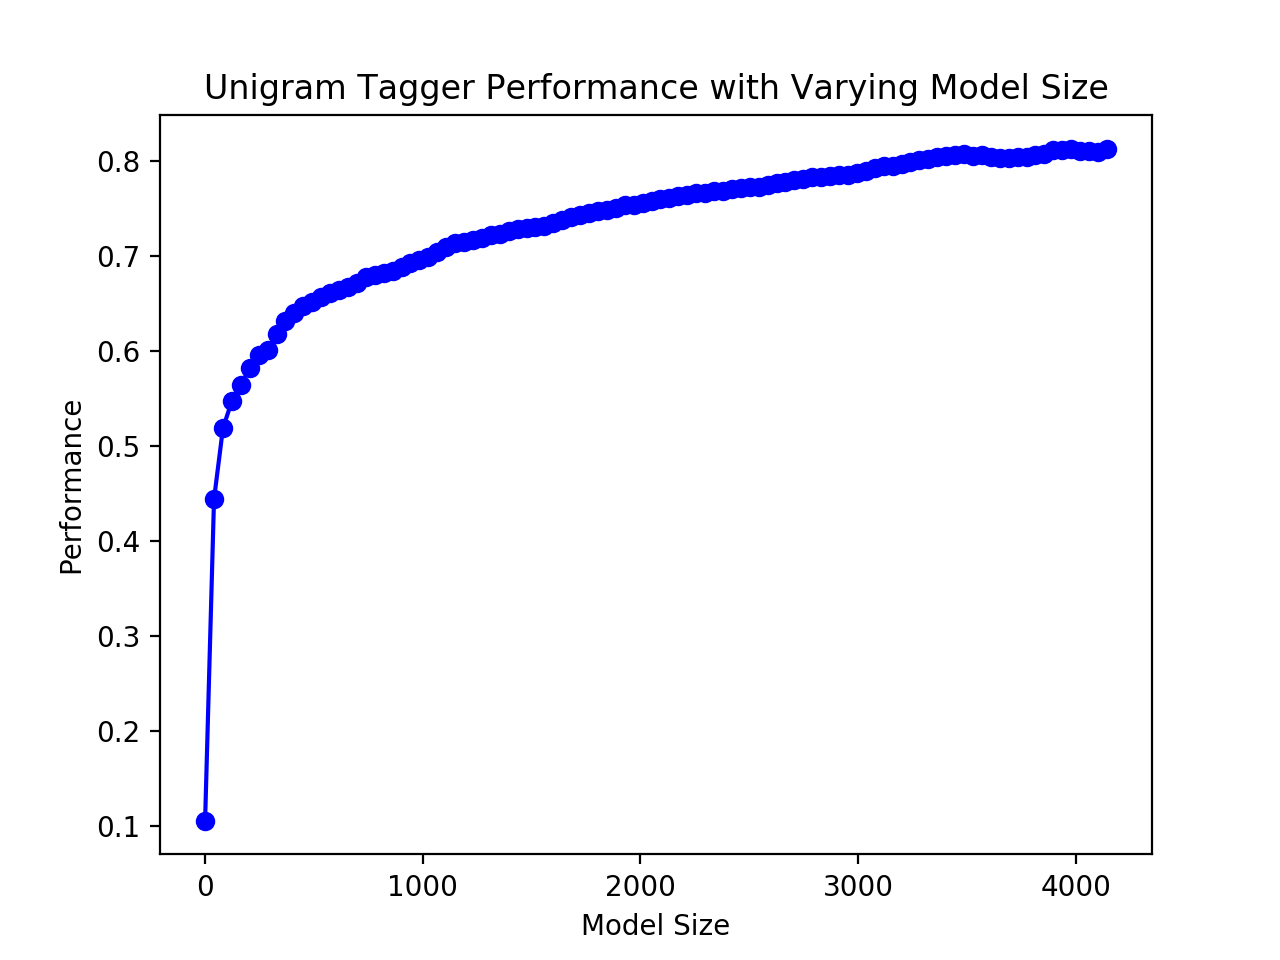
\includegraphics[width=550pt]{unigram_tagger_performance.png}
	
	Code for the tagger:
	
	\begin{lstlisting}
		import nltk
		import pylab
		from nltk.corpus import brown
		
		def performance_with_unigram_tagger(orig_data, size): 
			# Training data is from the start of data to the size value
			unigram_tagger = nltk.UnigramTagger(orig_data[:size])
			# Testing data is what's left after braking up training data
			return unigram_tagger.evaluate(orig_data[size:])
		
		def display():
			# Get our gold standard
			brown_tagged_sents = brown.tagged_sents(categories='news')
			# The number of sizes we want to test
			number_of_sizes = 100
			max_size = int(len(brown_tagged_sents) * 0.9)
			# get our list of sizes
			sizes_of_training = range(1, max_size, int(max_size / number_of_sizes)) 
			# Get a performance for each size
			perfs = [performance_with_unigram_tagger(brown_tagged_sents, size) for size in sizes_of_training]
			pylab.plot(sizes_of_training, perfs, '-bo')
			pylab.title('Unigram Tagger Performance with Varying Model Size')
			pylab.xlabel('Model Size')
			pylab.ylabel('Performance')
			pylab.show()
		
		if __name__ == '__main__': 
			display()
	\end{lstlisting}
	
\end{solution} 
\end{document}